\documentclass[10pt]{article}
\usepackage{graphicx}
\usepackage{float}
\usepackage{amsmath}
\usepackage{amscd}
\usepackage{hyperref}
\usepackage{enumerate}
\usepackage{amsfonts}
\usepackage{amssymb}
\usepackage[utf8]{inputenc}
\usepackage{amsthm}
\usepackage{booktabs}
\usepackage{subcaption}
\usepackage{listings}
\usepackage{lscape}
\usepackage{tikz}
\usepackage{color} %red, green, blue, yellow, cyan, magenta, black, white
\usepackage{xcolor}
\usepackage{fullpage}
\usetikzlibrary{calc}
\usepackage{multirow,array}


\newtheorem{theorem}{Theorem}
\newtheorem{lem}[theorem]{Lemma}
\newtheorem{dfn}{Definition}
\newtheorem{cor}[theorem]{Corollary}
\newtheorem{obs}{Obs}
\newtheorem{rem}{Remark}
\newtheorem{prob}{Problem}

\begin{document}


\title{`Toy Model'}

\author{ Moni Zamudio \and Isaac Meza}
\date{This draft: \today \\[2 cm] }

\maketitle


\subsection*{A Simple Game with Incomplete Information: Types and Beliefs}

\begin{dfn}[Game with incomplete information] A game with incomplete information $\mathcal{G}=(\Theta, S, P, u)$ consists of:
\begin{enumerate}[(i)]
\item A set $\Theta=\prod_{i\in I}\Theta_i$, where $\Theta_i$ is the finite set of possible types of player $i$ 
\item A set $S=\prod_{i\in I} S_i$, where $S_i$ is the set of possible strategies for player $i$
\item A joint probability distribution $p(\theta_1,\ldots, \theta_I)$ over types. For finite type space, we assume that $p(\theta_i)>0$ for all $\theta_i\in \Theta_i$
\item Payoff function $u_i:S\times \Theta\longmapsto \mathbb{R}$
\end{enumerate}
\end{dfn}

To study this type of games we rely on the idea by Harsanyi, assuming that the game begins with a move by nature which selects the different players’ preferences — or more generally, their types. So that the game can be thought as a \emph{complete} game but with \emph{imperfect information}
The type profile determines not only players’ payoffs but also their beliefs about other players’ types. Not everyone observes nature's move (player $i$ learns $\Theta_i$ but not $\Theta_{-i}$).\\

To analyze a game of incomplete information, we look at the \emph{Nash equilibrium} of the game where nature is a player. \\

A Bayesian pure strategy for player $i$ in $\mathcal{G}$ is a function from the possible set of types of player $i$ to the set of possible strategies.\\


\begin{dfn}[Bayesian-Nash equilibrium] A Bayesian strategy profile $(f_1,\ldots, f_I)$is a Bayesian-Nash equilibrium if for all $i$
\[f_i\in \text{argmax}_{f_{i}^{\prime}\in S_{i}^{\Theta_i}} \sum_{\theta\in \Theta} u_i\left(f_{i}^{\prime}(\theta_i), f_{-i}(\theta_{-i}),\theta_i, \theta_{-i}\right)p(\theta_i,\theta_{-i})\]
or alternatively, for all $i$, $\theta_i$ and $s_i$:
\[\sum_{\theta_{-i}\in \Theta_{-i}} u_i\left(f_{i}(\theta_i), f_{-i}(\theta_{-i}),\theta_i, \theta_{-i} \right) p(\theta_i|\theta_{-i})\geq \sum_{\theta_{-i}\in \Theta_{-i}} u_i\left(s_i, f_{-i}(\theta_{-i}),\theta_i, \theta_{-i} \right) p(\theta_i|\theta_{-i})\]
\end{dfn}

The second part of the definition just says that in order to maximize your expected payoff given that you know your types, then the strategy you choose for each type should maximize your payoff conditional on your having that type. Note that a Bayesian-Nash equilibrium is simply a Nash equilibrium in which nature moves first, chooses $\theta\in \Theta$ from a distribution with probability $p(\theta)$ and reveals $\theta_i$ to player $i$.\\

In the model introduced here, the source of uncertainty comes  as uncertainty about the types of players which translates as uncertainty in preferences and payoffs (the employee's lawyer (A)  and the employee (E) ) There can be 2 types of lawyers (Truthful and non-truthful) and 2 types of cases(High value and low value), which gives 4 settings. Payoffs are only known to the lawyer once he knows his type and the type of case. But because the players’ types are random and unknown to each other, they are uncertain about “who” their opponent is. However, they have the same beliefs about frequencies of opponent types.\\

Nature makes first move, choosing both the type of lawyer and type of case, the only one that knows this information is the lawyer. Once he knows his own type and the type of case, he sends a signal about the nature of the case (High value (H) / Low value (L) ) to the employee, and the latter makes the decision to sue (D) or not (N). \\

The 4 settings can be described as follows 

  \begin{table}[H]
  \begin{center}
    \setlength{\extrarowheight}{2pt}
    \begin{tabular}{*{4}{c|}}
      \multicolumn{2}{c}{} & \multicolumn{2}{c}{Player $E$}\\\cline{3-4}
      \multicolumn{1}{c}{} &  & $D$  & $ND$ \\\cline{2-4}
      \multirow{2}*{Player $A$}  & $H$ & $(1,x_1)$ & $(0,y_1)$ \\\cline{2-4}
      & $L$ & $(0,x_1)$ & $(0,y_1)$ \\\cline{2-4}
    \end{tabular}
            \begin{tabular}{*{4}{c|}}
      \multicolumn{2}{c}{} & \multicolumn{2}{c}{Player $E$}\\\cline{3-4}
      \multicolumn{1}{c}{} &  & $D$  & $ND$ \\\cline{2-4}
      \multirow{2}*{}  & $H$ & $(0,x_2)$ & $(0,y_2)$ \\\cline{2-4}
      & $L$ & $(0,x_2)$ & $(1,y_2)$ \\\cline{2-4}
    \end{tabular}
    \end{center}
  \end{table}
  
    \begin{table}[H]
      \begin{center}
    \setlength{\extrarowheight}{2pt}
        \begin{tabular}{*{4}{c|}}
      \multicolumn{2}{c}{} & \multicolumn{2}{c}{Player $E$}\\\cline{3-4}
      \multicolumn{1}{c}{} &  & $D$  & $ND$ \\\cline{2-4}
      \multirow{2}*{Player $A$}  & $H$ & $(1,x_3)$ & $(0,y_3)$ \\\cline{2-4}
      & $L$ & $(1,x_3)$ & $(0,y_3)$ \\\cline{2-4}
    \end{tabular}
        \begin{tabular}{*{4}{c|}}
      \multicolumn{2}{c}{} & \multicolumn{2}{c}{Player $E$}\\\cline{3-4}
      \multicolumn{1}{c}{} &  & $D$  & $ND$ \\\cline{2-4}
      \multirow{2}*{}  & $H$ & $(1,x_4)$ & $(0,y_4)$ \\\cline{2-4}
      & $L$ & $(1,x_4)$ & $(0,y_4)$ \\\cline{2-4}
    \end{tabular}
        \end{center}
   \footnotesize
    \textit{The 4 settings are respectively: Truthful-High value; Truthful-Low value; Non truthful-High value; Non truthful-Low value}         
  \end{table}

The rationale for the payoffs to be that way is intuitive. Consider the first game in which we have a truthful lawyer and a high value case, observe that lawyer has as dominant strategy to play $H$ and employee will be better off if he plays $D$ (sues), so that we impose the condition $x_1>y_1$. Note that $(H, D)$ corresponds to a Nash equilibrium, which is a desirable feature. In a similar fashion for the other 3 games we find that $x_2<y_2$, $x_3>y_3$ and $x_4<y_4$.\\

As the employee doesn't know in which of the 4 subgames she's actually in, the game can be described in extensive form as:
  
  
  
\begin{center}
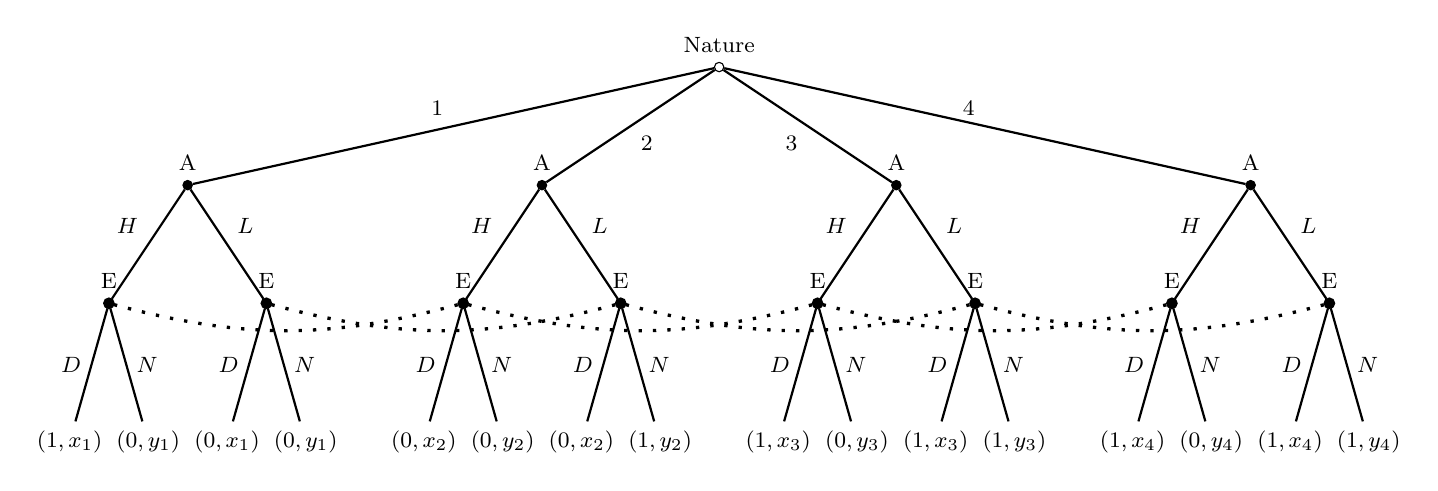
\begin{tikzpicture}[font=\footnotesize,edge from parent/.style={draw,thick}]
\label{geim}
% Two node styles: solid and hollow
\tikzstyle{solid node}=[circle,draw,inner sep=1.2,fill=black];
\tikzstyle{hollow node}=[circle,draw,inner sep=1.2];
% Specify spacing for each level of the tree
\tikzstyle{level 1}=[level distance=15mm,sibling distance=45mm]
\tikzstyle{level 2}=[level distance=15mm,sibling distance=20mm]
\tikzstyle{level 3}=[level distance=15mm,sibling distance=10mm]
% The Tree
\node(0)[hollow node ,label=above:{Nature}]{}
child{node[solid node,label=above:{A}]{}
child{node[solid node,label=above:{E}]{}
child{node[below]{$(1, x_1)$} edge from parent node[left]{$D$}}
child{node[below]{$(0,y_1)$} edge from parent node[right]{$N$}}
edge from parent node[above left]{$H$}
}
child{node[solid node,label=above:{E}]{}
child{node[below]{$(0,x_1)$} edge from parent node(s)[left]{$D$}}
child{node[below]{$(0,y_1)$} edge from parent node(N)[right]{$N$}}
edge from parent node[above right]{$L$}
}
edge from parent node[above left]{$1$}
}
child{node[solid node,label=above:{A}]{}
child{node[solid node,label=above:{E}]{}
child{node[below]{$(0,x_2)$} edge from parent node(m)[left]{$D$}}
child{node[below]{$(0,y_2)$} edge from parent node(n)[right]{$N$}}
edge from parent node[above left]{$H$}
}
child{node[solid node,label=above:{E}]{}
child{node[below]{$(0,x_2)$} edge from parent node[left]{$D$}}
child{node[below]{$(1,y_2)$} edge from parent node[right]{$N$}}
edge from parent node[above right]{$L$}
}
edge from parent node[below right]{$2$}
}
child{node[solid node,label=above:{A}]{}
child{node[solid node,label=above:{E}]{}
child{node[below]{$(1,x_3)$} edge from parent node[left]{$D$}}
child{node[below]{$(0,y_3)$} edge from parent node[right]{$N$}}
edge from parent node[above left]{$H$}
}
child{node[solid node,label=above:{E}]{}
child{node[below]{$(1,x_3)$} edge from parent node(D)[left]{$D$}}
child{node[below]{$(1,y_3)$} edge from parent node(N)[right]{$N$}}
edge from parent node[above right]{$L$}
}
edge from parent node[below left]{$3$}
}
child{node[solid node,label=above:{A}]{}
child{node[solid node,label=above:{E}]{}
child{node[below]{$(1,x_4)$} edge from parent node[left]{$D$}}
child{node[below]{$(0,y_4)$} edge from parent node[right]{$N$}}
edge from parent node[above left]{$H$}
}
child{node[solid node,label=above:{E}]{}
child{node[below]{$(1,x_4)$} edge from parent node(D)[left]{$D$}}
child{node[below]{$(1,y_4)$} edge from parent node(N)[right]{$N$}}
edge from parent node[above right]{$L$}
}
edge from parent node[above left]{$4$}
};
% information sets
\draw[loosely dotted,very thick](0-1-1)to[out=-15,in=195](0-2-1);
\draw[loosely dotted,very thick](0-1-2)to[out=-15,in=195](0-2-2);
\draw[loosely dotted,very thick](0-2-1)to[out=-15,in=195](0-3-1);
\draw[loosely dotted,very thick](0-2-2)to[out=-15,in=195](0-3-2);
\draw[loosely dotted,very thick](0-3-1)to[out=-15,in=195](0-4-1);
\draw[loosely dotted,very thick](0-3-2)to[out=-15,in=195](0-4-2);
% movers

\end{tikzpicture}
\end{center}


From the extensive form game we can deduce the payoffs to the 4 settings according to nature's choice. This is represented in the following tables:

\begin{table}[H]
\centering
\setlength\tabcolsep{4pt}
\begin{minipage}{0.48\textwidth}
\centering
        {% Table generated by Excel2LaTeX from sheet 'Hoja1'
\begin{tabular}{lrrrr}
\toprule
      & \multicolumn{1}{c}{DD} & \multicolumn{1}{c}{DN} & \multicolumn{1}{c}{ND} & \multicolumn{1}{c}{NN} \\
\midrule
HHHH  & \multicolumn{1}{l}{$( 1 , x_1 )$} & \multicolumn{1}{l}{$( 1 , x_1 )$} & \multicolumn{1}{l}{$( 0 , y_1 )$} & \multicolumn{1}{l}{$( 0 , y_1 )$} \\
HLHH  & \multicolumn{1}{l}{$( 1 , x_1 )$} & \multicolumn{1}{l}{$( 1 , x_1 )$} & \multicolumn{1}{l}{$( 0 , y_1 )$} & \multicolumn{1}{l}{$( 0 , y_1 )$} \\
HHLH  & \multicolumn{1}{l}{$( 1 , x_1 )$} & \multicolumn{1}{l}{$( 1 , x_1 )$} & \multicolumn{1}{l}{$( 0 , y_1 )$} & \multicolumn{1}{l}{$( 0 , y_1 )$} \\
HHHL  & \multicolumn{1}{l}{$( 1 , x_1 )$} & \multicolumn{1}{l}{$( 1 , x_1 )$} & \multicolumn{1}{l}{$( 0 , y_1 )$} & \multicolumn{1}{l}{$( 0 , y_1 )$} \\
HLLH  & \multicolumn{1}{l}{$( 1 , x_1 )$} & \multicolumn{1}{l}{$( 1 , x_1 )$} & \multicolumn{1}{l}{$( 0 , y_1 )$} & \multicolumn{1}{l}{$( 0 , y_1 )$} \\
HHLL  & \multicolumn{1}{l}{$( 1 , x_1 )$} & \multicolumn{1}{l}{$( 1 , x_1 )$} & \multicolumn{1}{l}{$( 0 , y_1 )$} & \multicolumn{1}{l}{$( 0 , y_1 )$} \\
HLHL  & \multicolumn{1}{l}{$( 1 , x_1 )$} & \multicolumn{1}{l}{$( 1 , x_1 )$} & \multicolumn{1}{l}{$( 0 , y_1 )$} & \multicolumn{1}{l}{$( 0 , y_1 )$} \\
HLLL  & \multicolumn{1}{l}{$( 1 , x_1 )$} & \multicolumn{1}{l}{$( 1 , x_1 )$} & \multicolumn{1}{l}{$( 0 , y_1 )$} & \multicolumn{1}{l}{$( 0 , y_1 )$} \\
LHHH  & \multicolumn{1}{l}{$( 0 , x_1 )$} & \multicolumn{1}{l}{$( 0 , y_1 )$} & \multicolumn{1}{l}{$( 0 , x_1 )$} & \multicolumn{1}{l}{$( 0 , y_1 )$} \\
LLHH  & \multicolumn{1}{l}{$( 0 , x_1 )$} & \multicolumn{1}{l}{$( 0 , y_1 )$} & \multicolumn{1}{l}{$( 0 , x_1 )$} & \multicolumn{1}{l}{$( 0 , y_1 )$} \\
LHLH  & \multicolumn{1}{l}{$( 0 , x_1 )$} & \multicolumn{1}{l}{$( 0 , y_1 )$} & \multicolumn{1}{l}{$( 0 , x_1 )$} & \multicolumn{1}{l}{$( 0 , y_1 )$} \\
LHHL  & \multicolumn{1}{l}{$( 0 , x_1 )$} & \multicolumn{1}{l}{$( 0 , y_1 )$} & \multicolumn{1}{l}{$( 0 , x_1 )$} & \multicolumn{1}{l}{$( 0 , y_1 )$} \\
LLLH  & \multicolumn{1}{l}{$( 0 , x_1 )$} & \multicolumn{1}{l}{$( 0 , y_1 )$} & \multicolumn{1}{l}{$( 0 , x_1 )$} & \multicolumn{1}{l}{$( 0 , y_1 )$} \\
LLHL  & \multicolumn{1}{l}{$( 0 , x_1 )$} & \multicolumn{1}{l}{$( 0 , y_1 )$} & \multicolumn{1}{l}{$( 0 , x_1 )$} & \multicolumn{1}{l}{$( 0 , y_1 )$} \\
LHLL  & \multicolumn{1}{l}{$( 0 , x_1 )$} & \multicolumn{1}{l}{$( 0 , y_1 )$} & \multicolumn{1}{l}{$( 0 , x_1 )$} & \multicolumn{1}{l}{$( 0 , y_1 )$} \\
LLLL  & \multicolumn{1}{l}{$( 0 , x_1 )$} & \multicolumn{1}{l}{$( 0 , y_1 )$} & \multicolumn{1}{l}{$( 0 , x_1 )$} & \multicolumn{1}{l}{$( 0 , y_1 )$} \\
\bottomrule
\end{tabular}%
}
\caption*{Payoff Matrix: Truthful Lawyer and High value case}
\label{PM1} 
\end{minipage}%
\hfill
\begin{minipage}{0.48\textwidth}
\centering
        {% Table generated by Excel2LaTeX from sheet 'Hoja1'
\begin{tabular}{lrrrr}
\toprule
      & \multicolumn{1}{c}{DD} & \multicolumn{1}{c}{DN} & \multicolumn{1}{c}{ND} & \multicolumn{1}{c}{NN} \\
\midrule
HHHH  & \multicolumn{1}{l}{$( 0 , x_2 )$} & \multicolumn{1}{l}{$( 0 , x_2 )$} & \multicolumn{1}{l}{$( 0 , y_2 )$} & \multicolumn{1}{l}{$( 0 , y_2 )$} \\
HLHH  & \multicolumn{1}{l}{$( 0 , x_2 )$} & \multicolumn{1}{l}{$( 1 , y_2 )$} & \multicolumn{1}{l}{$( 0 , x_2 )$} & \multicolumn{1}{l}{$( 1 , y_2 )$} \\
HHLH  & \multicolumn{1}{l}{$( 0 , x_2 )$} & \multicolumn{1}{l}{$( 0 , x_2 )$} & \multicolumn{1}{l}{$( 0 , y_2 )$} & \multicolumn{1}{l}{$( 0 , y_2 )$} \\
HHHL  & \multicolumn{1}{l}{$( 0 , x_2 )$} & \multicolumn{1}{l}{$( 0 , x_2 )$} & \multicolumn{1}{l}{$( 0 , y_2 )$} & \multicolumn{1}{l}{$( 0 , y_2 )$} \\
HLLH  & \multicolumn{1}{l}{$( 0 , x_2 )$} & \multicolumn{1}{l}{$( 1 , y_2 )$} & \multicolumn{1}{l}{$( 0 , x_2 )$} & \multicolumn{1}{l}{$( 1 , y_2 )$} \\
HHLL  & \multicolumn{1}{l}{$( 0 , x_2 )$} & \multicolumn{1}{l}{$( 0 , x_2 )$} & \multicolumn{1}{l}{$( 0 , y_2 )$} & \multicolumn{1}{l}{$( 0 , y_2 )$} \\
HLHL  & \multicolumn{1}{l}{$( 0 , x_2 )$} & \multicolumn{1}{l}{$( 1 , y_2 )$} & \multicolumn{1}{l}{$( 0 , x_2 )$} & \multicolumn{1}{l}{$( 1 , y_2 )$} \\
HLLL  & \multicolumn{1}{l}{$( 0 , x_2 )$} & \multicolumn{1}{l}{$( 1 , y_2 )$} & \multicolumn{1}{l}{$( 0 , x_2 )$} & \multicolumn{1}{l}{$( 1 , y_2 )$} \\
LHHH  & \multicolumn{1}{l}{$( 0 , x_2 )$} & \multicolumn{1}{l}{$( 0 , x_2 )$} & \multicolumn{1}{l}{$( 0 , y_2 )$} & \multicolumn{1}{l}{$( 0 , y_2 )$} \\
LLHH  & \multicolumn{1}{l}{$( 0 , x_2 )$} & \multicolumn{1}{l}{$( 1 , y_2 )$} & \multicolumn{1}{l}{$( 0 , x_2 )$} & \multicolumn{1}{l}{$( 1 , y_2 )$} \\
LHLH  & \multicolumn{1}{l}{$( 0 , x_2 )$} & \multicolumn{1}{l}{$( 0 , x_2 )$} & \multicolumn{1}{l}{$( 0 , y_2 )$} & \multicolumn{1}{l}{$( 0 , y_2 )$} \\
LHHL  & \multicolumn{1}{l}{$( 0 , x_2 )$} & \multicolumn{1}{l}{$( 0 , x_2 )$} & \multicolumn{1}{l}{$( 0 , y_2 )$} & \multicolumn{1}{l}{$( 0 , y_2 )$} \\
LLLH  & \multicolumn{1}{l}{$( 0 , x_2 )$} & \multicolumn{1}{l}{$( 1 , y_2 )$} & \multicolumn{1}{l}{$( 0 , x_2 )$} & \multicolumn{1}{l}{$( 1 , y_2 )$} \\
LLHL  & \multicolumn{1}{l}{$( 0 , x_2 )$} & \multicolumn{1}{l}{$( 1 , y_2 )$} & \multicolumn{1}{l}{$( 0 , x_2 )$} & \multicolumn{1}{l}{$( 1 , y_2 )$} \\
LHLL  & \multicolumn{1}{l}{$( 0 , x_2 )$} & \multicolumn{1}{l}{$( 0 , x_2 )$} & \multicolumn{1}{l}{$( 0 , y_2 )$} & \multicolumn{1}{l}{$( 0 , y_2 )$} \\
LLLL  & \multicolumn{1}{l}{$( 0 , x_2 )$} & \multicolumn{1}{l}{$( 1 , y_2 )$} & \multicolumn{1}{l}{$( 0 , x_2 )$} & \multicolumn{1}{l}{$( 1 , y_2 )$} \\
\bottomrule
\end{tabular}%
}
\caption*{Payoff Matrix: Truthful Lawyer and Low value case}
\label{PM2} 
\end{minipage}%
\end{table}


\begin{table}[H]
\centering
\setlength\tabcolsep{4pt}
\begin{minipage}{0.48\textwidth}
\centering
        {% Table generated by Excel2LaTeX from sheet 'Hoja1'
\begin{tabular}{lrrrr}
\toprule
      & \multicolumn{1}{c}{DD} & \multicolumn{1}{c}{DN} & \multicolumn{1}{c}{ND} & \multicolumn{1}{c}{NN} \\
\midrule
HHHH  & \multicolumn{1}{l}{$( 1 , x_3 )$} & \multicolumn{1}{l}{$( 1 , x_3 )$} & \multicolumn{1}{l}{$( 0 , y_3 )$} & \multicolumn{1}{l}{$( 0 , y_3 )$} \\
HLHH  & \multicolumn{1}{l}{$( 1 , x_3 )$} & \multicolumn{1}{l}{$( 1 , x_3 )$} & \multicolumn{1}{l}{$( 0 , y_3 )$} & \multicolumn{1}{l}{$( 0 , y_3 )$} \\
HHLH  & \multicolumn{1}{l}{$( 1 , x_3 )$} & \multicolumn{1}{l}{$( 0 , y_3 )$} & \multicolumn{1}{l}{$( 1 , x_3 )$} & \multicolumn{1}{l}{$( 0 , y_3 )$} \\
HHHL  & \multicolumn{1}{l}{$( 1 , x_3 )$} & \multicolumn{1}{l}{$( 1 , x_3 )$} & \multicolumn{1}{l}{$( 0 , y_3 )$} & \multicolumn{1}{l}{$( 0 , y_3 )$} \\
HLLH  & \multicolumn{1}{l}{$( 1 , x_3 )$} & \multicolumn{1}{l}{$( 0 , y_3 )$} & \multicolumn{1}{l}{$( 1 , x_3 )$} & \multicolumn{1}{l}{$( 0 , y_3 )$} \\
HHLL  & \multicolumn{1}{l}{$( 1 , x_3 )$} & \multicolumn{1}{l}{$( 0 , y_3 )$} & \multicolumn{1}{l}{$( 1 , x_3 )$} & \multicolumn{1}{l}{$( 0 , y_3 )$} \\
HLHL  & \multicolumn{1}{l}{$( 1 , x_3 )$} & \multicolumn{1}{l}{$( 1 , x_3 )$} & \multicolumn{1}{l}{$( 0 , y_3 )$} & \multicolumn{1}{l}{$( 0 , y_3 )$} \\
HLLL  & \multicolumn{1}{l}{$( 1 , x_3 )$} & \multicolumn{1}{l}{$( 0 , y_3 )$} & \multicolumn{1}{l}{$( 1 , x_3 )$} & \multicolumn{1}{l}{$( 0 , y_3 )$} \\
LHHH  & \multicolumn{1}{l}{$( 1 , x_3 )$} & \multicolumn{1}{l}{$( 1 , x_3 )$} & \multicolumn{1}{l}{$( 0 , y_3 )$} & \multicolumn{1}{l}{$( 0 , y_3 )$} \\
LLHH  & \multicolumn{1}{l}{$( 1 , x_3 )$} & \multicolumn{1}{l}{$( 1 , x_3 )$} & \multicolumn{1}{l}{$( 0 , y_3 )$} & \multicolumn{1}{l}{$( 0 , y_3 )$} \\
LHLH  & \multicolumn{1}{l}{$( 1 , x_3 )$} & \multicolumn{1}{l}{$( 0 , y_3 )$} & \multicolumn{1}{l}{$( 1 , x_3 )$} & \multicolumn{1}{l}{$( 0 , y_3 )$} \\
LHHL  & \multicolumn{1}{l}{$( 1 , x_3 )$} & \multicolumn{1}{l}{$( 1 , x_3 )$} & \multicolumn{1}{l}{$( 0 , y_3 )$} & \multicolumn{1}{l}{$( 0 , y_3 )$} \\
LLLH  & \multicolumn{1}{l}{$( 1 , x_3 )$} & \multicolumn{1}{l}{$( 0 , y_3 )$} & \multicolumn{1}{l}{$( 1 , x_3 )$} & \multicolumn{1}{l}{$( 0 , y_3 )$} \\
LLHL  & \multicolumn{1}{l}{$( 1 , x_3 )$} & \multicolumn{1}{l}{$( 1 , x_3 )$} & \multicolumn{1}{l}{$( 0 , y_3 )$} & \multicolumn{1}{l}{$( 0 , y_3 )$} \\
LHLL  & \multicolumn{1}{l}{$( 1 , x_3 )$} & \multicolumn{1}{l}{$( 0 , y_3 )$} & \multicolumn{1}{l}{$( 1 , x_3 )$} & \multicolumn{1}{l}{$( 0 , y_3 )$} \\
LLLL  & \multicolumn{1}{l}{$( 1 , x_3 )$} & \multicolumn{1}{l}{$( 0 , y_3 )$} & \multicolumn{1}{l}{$( 1 , x_3 )$} & \multicolumn{1}{l}{$( 0 , y_3 )$} \\
\bottomrule
\end{tabular}%
}
\caption*{Payoff Matrix: Non-truthful Lawyer and High value case}
\label{PM3} 
\end{minipage}%
\hfill
\begin{minipage}{0.48\textwidth}
\centering
        {% Table generated by Excel2LaTeX from sheet 'Hoja1'
\begin{tabular}{lrrrr}
\toprule
      & \multicolumn{1}{c}{DD} & \multicolumn{1}{c}{DN} & \multicolumn{1}{c}{ND} & \multicolumn{1}{c}{NN} \\
\midrule
HHHH  & \multicolumn{1}{l}{$( 1 , x_4 )$} & \multicolumn{1}{l}{$( 1 , x_4 )$} & \multicolumn{1}{l}{$( 0 , y_4 )$} & \multicolumn{1}{l}{$( 0 , y_4 )$} \\
HLHH  & \multicolumn{1}{l}{$( 1 , x_4 )$} & \multicolumn{1}{l}{$( 1 , x_4 )$} & \multicolumn{1}{l}{$( 0 , y_4 )$} & \multicolumn{1}{l}{$( 0 , y_4 )$} \\
HHLH  & \multicolumn{1}{l}{$( 1 , x_4 )$} & \multicolumn{1}{l}{$( 1 , x_4 )$} & \multicolumn{1}{l}{$( 0 , y_4 )$} & \multicolumn{1}{l}{$( 0 , y_4 )$} \\
HHHL  & \multicolumn{1}{l}{$( 1 , x_4 )$} & \multicolumn{1}{l}{$( 0 , y_4 )$} & \multicolumn{1}{l}{$( 1 , x_4 )$} & \multicolumn{1}{l}{$( 0 , y_4 )$} \\
HLLH  & \multicolumn{1}{l}{$( 1 , x_4 )$} & \multicolumn{1}{l}{$( 1 , x_4 )$} & \multicolumn{1}{l}{$( 0 , y_4 )$} & \multicolumn{1}{l}{$( 0 , y_4 )$} \\
HHLL  & \multicolumn{1}{l}{$( 1 , x_4 )$} & \multicolumn{1}{l}{$( 0 , y_4 )$} & \multicolumn{1}{l}{$( 1 , x_4 )$} & \multicolumn{1}{l}{$( 0 , y_4 )$} \\
HLHL  & \multicolumn{1}{l}{$( 1 , x_4 )$} & \multicolumn{1}{l}{$( 0 , y_4 )$} & \multicolumn{1}{l}{$( 1 , x_4 )$} & \multicolumn{1}{l}{$( 0 , y_4 )$} \\
HLLL  & \multicolumn{1}{l}{$( 1 , x_4 )$} & \multicolumn{1}{l}{$( 0 , y_4 )$} & \multicolumn{1}{l}{$( 1 , x_4 )$} & \multicolumn{1}{l}{$( 0 , y_4 )$} \\
LHHH  & \multicolumn{1}{l}{$( 1 , x_4 )$} & \multicolumn{1}{l}{$( 1 , x_4 )$} & \multicolumn{1}{l}{$( 0 , y_4 )$} & \multicolumn{1}{l}{$( 0 , y_4 )$} \\
LLHH  & \multicolumn{1}{l}{$( 1 , x_4 )$} & \multicolumn{1}{l}{$( 1 , x_4 )$} & \multicolumn{1}{l}{$( 0 , y_4 )$} & \multicolumn{1}{l}{$( 0 , y_4 )$} \\
LHLH  & \multicolumn{1}{l}{$( 1 , x_4 )$} & \multicolumn{1}{l}{$( 1 , x_4 )$} & \multicolumn{1}{l}{$( 0 , y_4 )$} & \multicolumn{1}{l}{$( 0 , y_4 )$} \\
LHHL  & \multicolumn{1}{l}{$( 1 , x_4 )$} & \multicolumn{1}{l}{$( 0 , y_4 )$} & \multicolumn{1}{l}{$( 1 , x_4 )$} & \multicolumn{1}{l}{$( 0 , y_4 )$} \\
LLLH  & \multicolumn{1}{l}{$( 1 , x_4 )$} & \multicolumn{1}{l}{$( 1 , x_4 )$} & \multicolumn{1}{l}{$( 0 , y_4 )$} & \multicolumn{1}{l}{$( 0 , y_4 )$} \\
LLHL  & \multicolumn{1}{l}{$( 1 , x_4 )$} & \multicolumn{1}{l}{$( 0 , y_4 )$} & \multicolumn{1}{l}{$( 1 , x_4 )$} & \multicolumn{1}{l}{$( 0 , y_4 )$} \\
LHLL  & \multicolumn{1}{l}{$( 1 , x_4 )$} & \multicolumn{1}{l}{$( 0 , y_4 )$} & \multicolumn{1}{l}{$( 1 , x_4 )$} & \multicolumn{1}{l}{$( 0 , y_4 )$} \\
LLLL  & \multicolumn{1}{l}{$( 1 , x_4 )$} & \multicolumn{1}{l}{$( 0 , y_4 )$} & \multicolumn{1}{l}{$( 1 , x_4 )$} & \multicolumn{1}{l}{$( 0 , y_4 )$} \\
\bottomrule
\end{tabular}%
}
\caption*{Payoff Matrix: Non-truthful Lawyer and Low value case}
\label{PM4} 
\end{minipage}%
\end{table}

The actual payoff matrix is the weighted sum of each of the 4 settings, which gives

\begin{table}[H]
\centering
        {% Table generated by Excel2LaTeX from sheet 'Hoja1'
\begin{tabular}{rrr}
\toprule
\toprule
      & \multicolumn{1}{c}{\colorbox{red}{DD}} & \multicolumn{1}{c}{\colorbox{red}{DN}} \\
\midrule
\multicolumn{1}{l}{\colorbox{blue}{HHHH}} & \multicolumn{1}{l}{\colorbox{yellow}{$( p_1+p_3+p_4\;\; ,\;\; p_1x_1+p_2x_2+p_3x_3+p_4x_4 )$}} & \multicolumn{1}{l}{$( p_1+p_3+p_4\;\; ,\;\; p_1x_1+p_2x_2+p_3x_3+p_4x_4 )$} \\
\multicolumn{1}{l}{\colorbox{blue}{HLHH}} & \multicolumn{1}{l}{$( p_1+p_3+p_4\;\; ,\;\; p_1x_1+p_2x_2+p_3x_3+p_4x_4 )$} & \multicolumn{1}{l}{\colorbox{yellow}{$( p_1+p_2+p_3+p_4\;\; ,\;\; p_1x_1+p_2y_2+p_3x_3+p_4x_4 )$}} \\
\multicolumn{1}{l}{\colorbox{blue}{HHLH}} & \multicolumn{1}{l}{\colorbox{yellow}{$( p_1+p_3+p_4\;\; ,\;\; p_1x_1+p_2x_2+p_3x_3+p_4x_4 )$}} & \multicolumn{1}{l}{$( p_1+p_4\;\; ,\;\; p_1x_1+p_2x_2+p_3y_3+p_4x_4 )$} \\
\multicolumn{1}{l}{HHHL} & \multicolumn{1}{l}{$( p_1+p_3+p_4\;\; ,\;\; p_1x_1+p_2x_2+p_3x_3+p_4x_4 )$} & \multicolumn{1}{l}{$( p_1+p_3\;\; ,\;\; p_1x_1+p_2x_2+p_3x_3+p_4y_4 )$} \\
\multicolumn{1}{l}{\colorbox{blue}{HLLH}} & \multicolumn{1}{l}{\colorbox{yellow}{$( p_1+p_3+p_4\;\; ,\;\; p_1x_1+p_2x_2+p_3x_3+p_4x_4 )$}} & \multicolumn{1}{l}{$( p_1+p_2+p_4\;\; ,\;\; p_1x_1+p_2y_2+p_3y_3+p_4x_4 )$} \\
\multicolumn{1}{l}{HHLL} & \multicolumn{1}{l}{$( p_1+p_3+p_4\;\; ,\;\; p_1x_1+p_2x_2+p_3x_3+p_4x_4 )$} & \multicolumn{1}{l}{$( p_1\;\; ,\;\; p_1x_1+p_2x_2+p_3y_3+p_4y_4 )$} \\
\multicolumn{1}{l}{HLHL} & \multicolumn{1}{l}{$( p_1+p_3+p_4\;\; ,\;\; p_1x_1+p_2x_2+p_3x_3+p_4x_4 )$} & \multicolumn{1}{l}{$( p_1+p_2+p_3\;\; ,\;\; p_1x_1+p_2y_2+p_3x_3+p_4y_4 )$} \\
\multicolumn{1}{l}{HLLL} & \multicolumn{1}{l}{$( p_1+p_3+p_4\;\; ,\;\; p_1x_1+p_2x_2+p_3x_3+p_4x_4 )$} & \multicolumn{1}{l}{$( p_1+p_2\;\; ,\;\; p_1x_1+p_2y_2+p_3y_3+p_4y_4 )$} \\
\multicolumn{1}{l}{\colorbox{blue}{LHHH}} & \multicolumn{1}{l}{$( p_3+p_4\;\; ,\;\; p_1x_1+p_2x_2+p_3x_3+p_4x_4 )$} & \multicolumn{1}{l}{$( p_3+p_4\;\; ,\;\; p_1y_1+p_2x_2+p_3x_3+p_4x_4 )$} \\
\multicolumn{1}{l}{\colorbox{blue}{LLHH}} & \multicolumn{1}{l}{$( p_3+p_4\;\; ,\;\; p_1x_1+p_2x_2+p_3x_3+p_4x_4 )$} & \multicolumn{1}{l}{$( p_2+p_3+p_4\;\; ,\;\; p_1y_1+p_2y_2+p_3x_3+p_4x_4 )$} \\
\multicolumn{1}{l}{\colorbox{blue}{LHLH}} & \multicolumn{1}{l}{$( p_3+p_4\;\; ,\;\; p_1x_1+p_2x_2+p_3x_3+p_4x_4 )$} & \multicolumn{1}{l}{$( p_4\;\; ,\;\; p_1y_1+p_2x_2+p_3y_3+p_4x_4 )$} \\
\multicolumn{1}{l}{LHHL} & \multicolumn{1}{l}{$( p_3+p_4\;\; ,\;\; p_1x_1+p_2x_2+p_3x_3+p_4x_4 )$} & \multicolumn{1}{l}{$( p_3\;\; ,\;\; p_1y_1+p_2x_2+p_3x_3+p_4y_4 )$} \\
\multicolumn{1}{l}{\colorbox{blue}{LLLH}} & \multicolumn{1}{l}{$( p_3+p_4\;\; ,\;\; p_1x_1+p_2x_2+p_3x_3+p_4x_4 )$} & \multicolumn{1}{l}{$( p_2+p_4\;\; ,\;\; p_1y_1+p_2y_2+p_3y_3+p_4x_4 )$} \\
\multicolumn{1}{l}{LLHL} & \multicolumn{1}{l}{$( p_3+p_4\;\; ,\;\; p_1x_1+p_2x_2+p_3x_3+p_4x_4 )$} & \multicolumn{1}{l}{$( p_2+p_3\;\; ,\;\; p_1y_1+p_2y_2+p_3x_3+p_4y_4 )$} \\
\multicolumn{1}{l}{LHLL} & \multicolumn{1}{l}{$( p_3+p_4\;\; ,\;\; p_1x_1+p_2x_2+p_3x_3+p_4x_4 )$} & \multicolumn{1}{l}{$( 0\;\; ,\;\; p_1y_1+p_2x_2+p_3y_3+p_4y_4 )$} \\
\multicolumn{1}{l}{LLLL} & \multicolumn{1}{l}{$( p_3+p_4\;\; ,\;\; p_1x_1+p_2x_2+p_3x_3+p_4x_4 )$} & \multicolumn{1}{l}{$( p_2\;\; ,\;\; p_1y_1+p_2y_2+p_3y_3+p_4y_4 )$} \\
      &       &  \\
      \toprule
      \toprule
      & \multicolumn{1}{c}{ND} & \multicolumn{1}{c}{NN} \\
      \midrule
\multicolumn{1}{l}{HHHH} & \multicolumn{1}{l}{$( 0\;\; ,\;\; p_1y_1+p_2y_2+p_3y_3+p_4y_4 )$} & \multicolumn{1}{l}{$( 0\;\; ,\;\; p_1y_1+p_2y_2+p_3y_3+p_4y_4 )$} \\
\multicolumn{1}{l}{HLHH} & \multicolumn{1}{l}{$( 0\;\; ,\;\; p_1y_1+p_2x_2+p_3y_3+p_4y_4 )$} & \multicolumn{1}{l}{$( p_2\;\; ,\;\; p_1y_1+p_2y_2+p_3y_3+p_4y_4 )$} \\
\multicolumn{1}{l}{HHLH} & \multicolumn{1}{l}{$( p_3\;\; ,\;\; p_1y_1+p_2y_2+p_3x_3+p_4y_4 )$} & \multicolumn{1}{l}{$( 0\;\; ,\;\; p_1y_1+p_2y_2+p_3y_3+p_4y_4 )$} \\
\multicolumn{1}{l}{HHHL} & \multicolumn{1}{l}{$( p_4\;\; ,\;\; p_1y_1+p_2y_2+p_3y_3+p_4x_4 )$} & \multicolumn{1}{l}{$( 0\;\; ,\;\; p_1y_1+p_2y_2+p_3y_3+p_4y_4 )$} \\
\multicolumn{1}{l}{HLLH} & \multicolumn{1}{l}{$( p_3\;\; ,\;\; p_1y_1+p_2x_2+p_3x_3+p_4y_4 )$} & \multicolumn{1}{l}{$( p_2\;\; ,\;\; p_1y_1+p_2y_2+p_3y_3+p_4y_4 )$} \\
\multicolumn{1}{l}{HHLL} & \multicolumn{1}{l}{$( p_3+p_4\;\; ,\;\; p_1y_1+p_2y_2+p_3x_3+p_4x_4 )$} & \multicolumn{1}{l}{$( 0\;\; ,\;\; p_1y_1+p_2y_2+p_3y_3+p_4y_4 )$} \\
\multicolumn{1}{l}{HLHL} & \multicolumn{1}{l}{$( p_4\;\; ,\;\; p_1y_1+p_2x_2+p_3y_3+p_4x_4 )$} & \multicolumn{1}{l}{$( p_2\;\; ,\;\; p_1y_1+p_2y_2+p_3y_3+p_4y_4 )$} \\
\multicolumn{1}{l}{HLLL} & \multicolumn{1}{l}{$( p_3+p_4\;\; ,\;\; p_1y_1+p_2x_2+p_3x_3+p_4x_4 )$} & \multicolumn{1}{l}{$( p_2\;\; ,\;\; p_1y_1+p_2y_2+p_3y_3+p_4y_4 )$} \\
\multicolumn{1}{l}{LHHH} & \multicolumn{1}{l}{$( 0\;\; ,\;\; p_1x_1+p_2y_2+p_3y_3+p_4y_4 )$} & \multicolumn{1}{l}{$( 0\;\; ,\;\; p_1y_1+p_2y_2+p_3y_3+p_4y_4 )$} \\
\multicolumn{1}{l}{LLHH} & \multicolumn{1}{l}{$( 0\;\; ,\;\; p_1x_1+p_2x_2+p_3y_3+p_4y_4 )$} & \multicolumn{1}{l}{$( p_2\;\; ,\;\; p_1y_1+p_2y_2+p_3y_3+p_4y_4 )$} \\
\multicolumn{1}{l}{LHLH} & \multicolumn{1}{l}{$( p_3\;\; ,\;\; p_1x_1+p_2y_2+p_3x_3+p_4y_4 )$} & \multicolumn{1}{l}{$( 0\;\; ,\;\; p_1y_1+p_2y_2+p_3y_3+p_4y_4 )$} \\
\multicolumn{1}{l}{LHHL} & \multicolumn{1}{l}{$( p_4\;\; ,\;\; p_1x_1+p_2y_2+p_3y_3+p_4x_4 )$} & \multicolumn{1}{l}{$( 0\;\; ,\;\; p_1y_1+p_2y_2+p_3y_3+p_4y_4 )$} \\
\multicolumn{1}{l}{LLLH} & \multicolumn{1}{l}{$( p_3\;\; ,\;\; p_1x_1+p_2x_2+p_3x_3+p_4y_4 )$} & \multicolumn{1}{l}{$( p_2\;\; ,\;\; p_1y_1+p_2y_2+p_3y_3+p_4y_4 )$} \\
\multicolumn{1}{l}{LLHL} & \multicolumn{1}{l}{$( p_4\;\; ,\;\; p_1x_1+p_2x_2+p_3y_3+p_4x_4 )$} & \multicolumn{1}{l}{$( p_2\;\; ,\;\; p_1y_1+p_2y_2+p_3y_3+p_4y_4 )$} \\
\multicolumn{1}{l}{LHLL} & \multicolumn{1}{l}{$( p_3+p_4\;\; ,\;\; p_1x_1+p_2y_2+p_3x_3+p_4x_4 )$} & \multicolumn{1}{l}{$( 0\;\; ,\;\; p_1y_1+p_2y_2+p_3y_3+p_4y_4 )$} \\
\multicolumn{1}{l}{LLLL} & \multicolumn{1}{l}{$( p_3+p_4\;\; ,\;\; p_1x_1+p_2x_2+p_3x_3+p_4x_4 )$} & \multicolumn{1}{l}{$( p_2\;\; ,\;\; p_1y_1+p_2y_2+p_3y_3+p_4y_4 )$} \\
\bottomrule
\bottomrule
\end{tabular}%
}
   \caption*{Payoff Matrix: Expected payoff matrix}
\end{table}

It is this last payoff matrix which we analyze to find pure Nash equilibrium. Highlighted in blue find the strategies of the lawyer where he sends the signal $H$ even though the case is a low value one, and highlighted in red the employee's strategies where he sues (D) when he is told $H$. We highlight in yellow the payoffs (and therefore the strategy profiles) that arise as Nash equilibrium, when the following conditions are satisfied:

\begin{enumerate}
    \item [$(HHHH, DD)$] $\sum p_i x_i\geq \sum p_i y_i $
    \item [$(HLHH, DN)$] $p_1x_1+p_2y_2+p_3x_3+p_4x_4\geq \sum p_iy_i$
    \item [$(HHLH, DD)$] $\sum p_i x_i \geq p_1y_1+p_2y_2+p_3x_3+p_4y_4$
    \item [$(HLLH, DD)$] $\sum p_i x_i \geq \sum p_i y_i$ 
    
    $\sum p_i x_i \geq  p_1y_1+p_2x_2+p_3x_3+p_4y_4$ 
    
    $\sum p_i x_i \geq p1_x1+p_2y_2+p_3y_3+p_4x_4$ 
\end{enumerate}


In the past profiles, the lawyer `cheats' the employee making him believe he has a high value case and so he sues. Note that this depends on the proportion of truthful lawyers and high value cases (the $p_i$'s). \\



%
%\pagebreak
%\pagenumbering{gobble}
%\nocite{*}
%\bibliography{bibliography}
%\bibliographystyle{plain}

\end{document}